\documentclass[11pt, oneside]{article} 
\usepackage{geometry}
\geometry{letterpaper} 
\usepackage{graphicx}
	
\usepackage{amssymb}
\usepackage{amsmath}
\usepackage{parskip}
\usepackage{color}
\usepackage{hyperref}

\graphicspath{{/Users/telliott/Github/calculus_book/png/}}
% \begin{center} 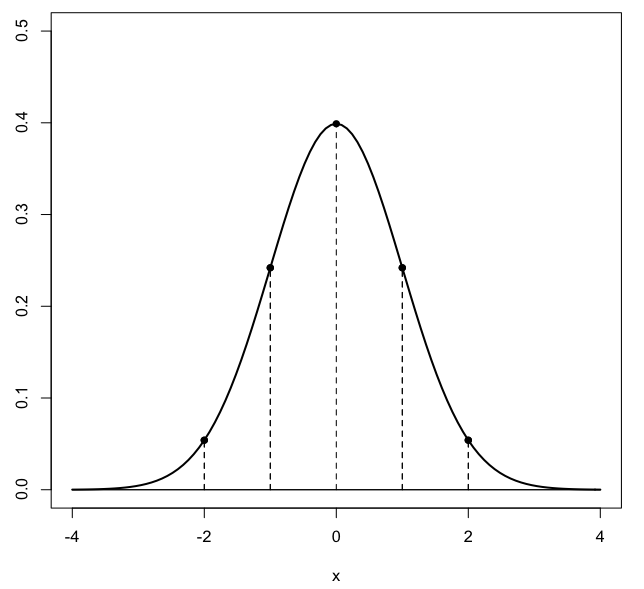
\includegraphics [scale=0.4] {gauss3.png} \end{center}

\title{Isosceles backward}
\date{}

\begin{document}
\maketitle
\Large

\subsection*{Prop. I.5}

\begin{quote}In isosceles triangles the angles at the base equal one another, and, if the equal straight lines are produced further, then the angles under the base equal one another.\end{quote}

\begin{center} 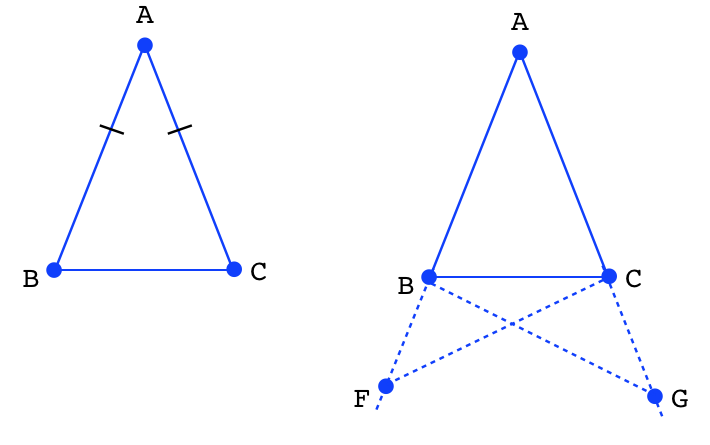
\includegraphics [scale=0.3] {PI_5a.png} \end{center}

We are given that $AB = AC$.  Extend the sides downward to $D$ and $E$ (not shown) and mark off equal distances $AF = AG$.

$\circ$ \ (0) given that $AB = AC$ and $AF = AG$

$\circ$ \ (1) $\triangle ACF \cong \triangle ABG$ [by SAS]

\begin{center} 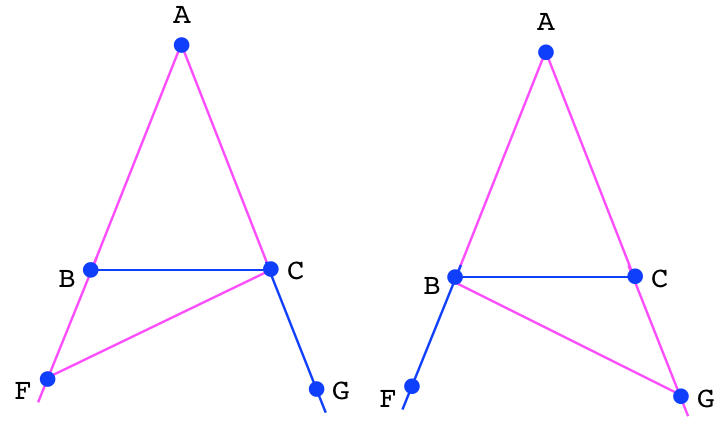
\includegraphics [scale=0.3] {PI_5b.png} \end{center}

$\circ$ \ (2) $\angle ACF = \angle ABG$ and $FC = BG$ [by congruent $\triangle$ from (1)]

$\circ$ \ (3) Further, $BF = CB$ [by subtraction, using (0)].

$\circ$ \ (4) $\triangle BCF \cong BCG$ by SSS.

\begin{center} 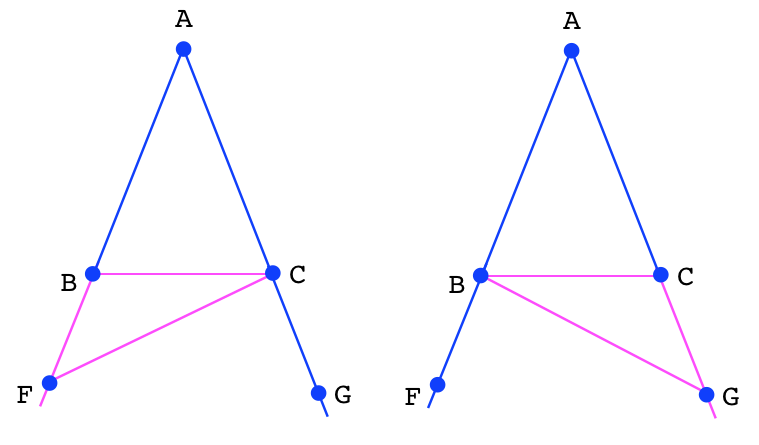
\includegraphics [scale=0.3] {PI_5c.png} \end{center}

$\circ$ \ (5) $\angle FBC = \angle BCG$ by congruent $\triangle$ in (4).

At this point we would use supplementary angles to finish the proof, but Euclid does not allow himself to do that.

$\circ$ \ (5) $\angle BCF = \angle CBG$ by congruent $\triangle$ from (4)

$\circ$ \ (7) $\angle ABG - \angle CBG = \angle ABC$.

$\circ$ \ (8) $\angle ACF - \angle BCF = \angle ACB$.

$\circ$ \ (9) But $\angle ABG = \angle ACF$ (2) and $\angle BCF = \angle CBG$ (5), so by subtraction we obtain equals and therefore have
\[ \angle ABC = \angle ACB \]

$\square$

\label{sec:isosceles_backward}

$\circ$  The base angles of an isosceles triangle are equal.  Also, if the two base angles are equal, the triangle is isosceles.

Euclid's proof is here:

\begin{center} 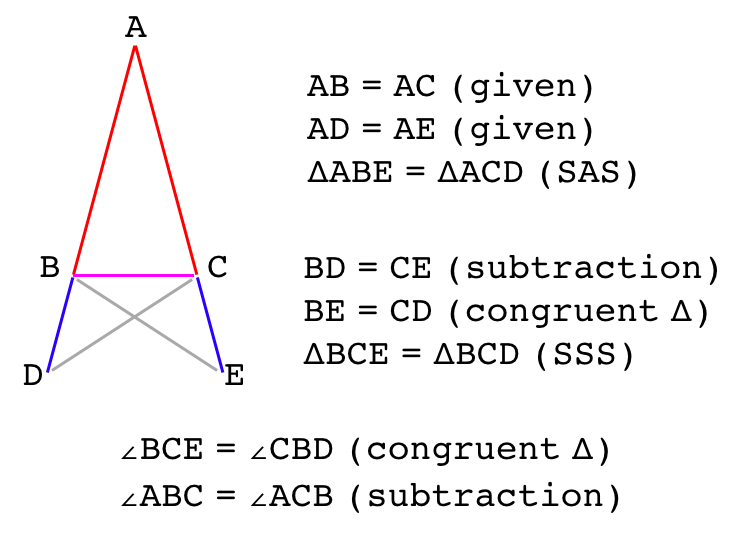
\includegraphics [scale=0.5] {isosceles_proof.png} \end{center}

Sometimes proofs can get a little complicated.  

The theorem says that the base angles are equal $\iff$ the two sides sides (not the base) are equal.  We proved that equal sides lead to equal angles, now we must proceed backwards, from equal angles to equal sides:

\begin{center} 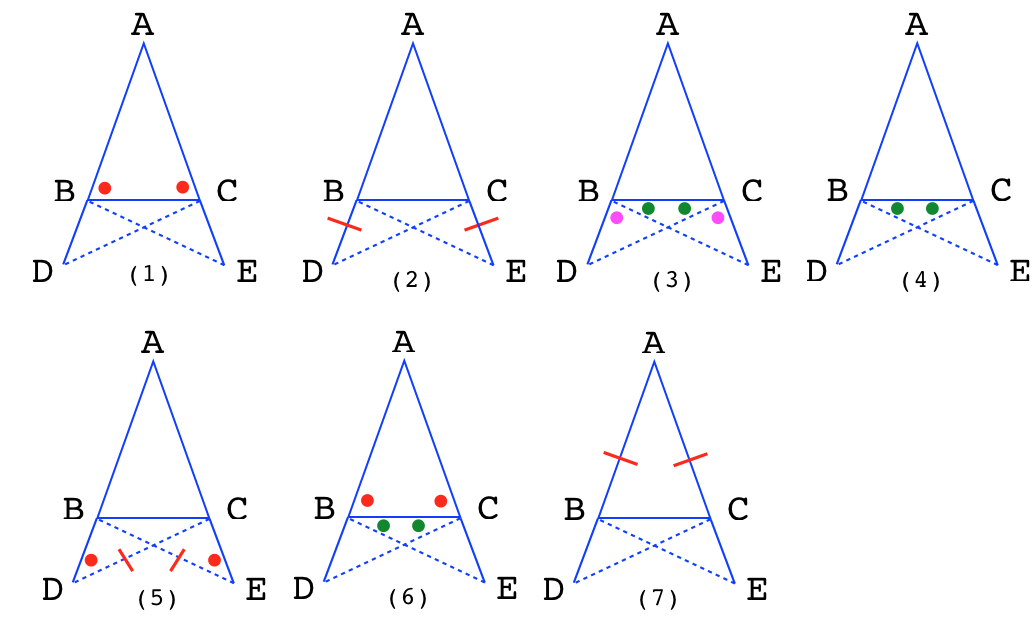
\includegraphics [scale=0.4] {isosceles5.png} \end{center}

$\circ$ \ $\angle ABC = \angle ACB$, given, (1)

$\circ$ \ $BD =CE$, by construction, (2)

$\circ$ \ $\angle DBC = \angle BCE$, supplementary angles, (3)

$\circ$ \ $\triangle DBC = \triangle BCE$, S-A-S, (3)

$\circ$ \ $\angle BCD = \angle CBE$, congruent triangles (4)

$\circ$ \ $\angle ADC = \angle AEB$, congruent triangles (5)

$\circ$ \ $BE = CD$, congruent triangles (5)

$\circ$ \ $\angle ADC = \angle ABE$, angle addition

$\circ$ \ $\triangle ADC = \triangle ABE$, A-S-A

$\circ$ \ $AB = AC$, congruent triangles

$\square$


\end{document}